\documentclass[UTF8,a4paper,12pt]{ctexbook} 

 \usepackage{graphicx}%学习插入图
 \usepackage{verbatim}%学习注释多行
 \usepackage{booktabs}%表格
 \usepackage{geometry}%图片
 \usepackage{amsmath}
 \usepackage{amssymb}
 \usepackage{listings}%代码
 \usepackage{xcolor}  %颜色
 \usepackage{enumitem}%列表格式
 \usepackage{tcolorbox}
 \usepackage{algorithm}  %format of the algorithm
 \usepackage{algorithmic}%format of the algorithm
 \usepackage{multirow}   %multirow for format of table
 \usepackage{tabularx} 	%表格排版格式控制
 \usepackage{array}	%表格排版格式控制
 \usepackage{hyperref} %超链接 \url{URL}
 \CTEXsetup[format+={\flushleft}]{section}
  %%%% 下面的命令添加新字体 %%%%%
  
 \renewcommand{\figurename}{Fig}
 
 \geometry{left=1.6cm,right=1.8cm,top=2cm,bottom=1.7cm} %设置文章宽度
 
 \pagestyle{plain} 		  %设置页面布局

 %代码效果定义
 \definecolor{mygreen}{rgb}{0,0.6,0}
 \definecolor{mygray}{rgb}{0.5,0.5,0.5}
 \definecolor{mymauve}{rgb}{0.58,0,0.82}
 \lstset{ %
 	backgroundcolor=\color{white},   % choose the background color
 	basicstyle=\footnotesize\ttfamily,        % size of fonts used for the code
 	%stringstyle=\color{codepurple},
 	%basicstyle=\footnotesize,
 	%breakatwhitespace=false,         
 	%breaklines=true,                 
 	%captionpos=b,                    
 	%keepspaces=true,                 
 	%numbers=left,                    
 	%numbersep=5pt,                  
 	%showspaces=false,                
 	%showstringspaces=false,
 	%showtabs=false,        
 	columns=fullflexible,
 	breaklines=true,                 % automatic line breaking only at whitespace
 	captionpos=b,                    % sets the caption-position to bottom
 	tabsize=4,
 	commentstyle=\color{mygreen},    % comment style
 	escapeinside={\%*}{*)},          % if you want to add LaTeX within your code
 	keywordstyle=\color{blue},       % keyword style
 	stringstyle=\color{mymauve}\ttfamily,     % string literal style
	%frame=single,					%tb top and bottom; L left double line
	xleftmargin=.02\textwidth, 
	%xrightmargin=.1\textwidth,
 	rulesepcolor=\color{red!20!green!20!blue!20},
 	% identifierstyle=\color{red},
 	language=c++,
 }
	
 \author{\kaishu 郑华}
 \title{\heiti Git 版本控制}
 
\begin{document}          %正文排版开始
 	\maketitle
 	\tableofcontents
  \chapter{Git 简介}
	  \section{集中式 版本控制系统SVN}
		  先说集中式版本控制系统,版本库是集中存放在中央服务器的,而干活的时候,用的都是自己的电脑,所以要先从中央服务器取得最新的版本,然后开始干活,干完活了,再把自己的活推送给中央服务器。\textbf{中央服务器就好比是一个图书馆,你要改一本书,必须先从图书馆借出来,然后回到家自己改,改完了,再放回图书馆}
			  
		   \begin{figure}[h]
		   	\centering
		   	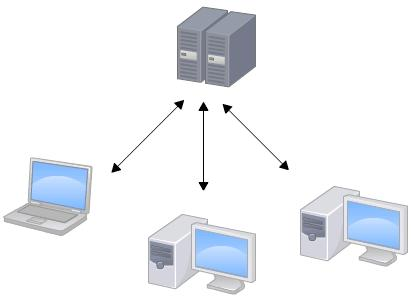
\includegraphics[scale = 0.7]{JiZhong.jpg}
		   	\caption{集中式架构结构图}
		   \end{figure}
		   
		  集中式版本控制系统最大的毛病就是必须联网才能工作,如果在局域网内还好,带宽够大,速度够快,可如果在互联网上,遇到网速慢的话,可能提交一个10M的文件就需要5分钟,这还不得把人给憋死啊
		  
	  \section{分布式 版本控制系统Git}
		  那分布式版本控制系统与集中式版本控制系统有何不同呢?首先,分布式版本控制系统根本没有“中央服务器”,\textbf{每个人的电脑上都是一个完整的版本库,这样,你工作的时候,就不需要联网了,因为版本库就在你自己的电脑上。既然每个人电脑上都有一个完整的版本库,那多个人如何协作呢?比方说你在自己电脑上改了文件A,你的同事也在他的电脑上改了文件A,这时,你们俩之间只需把各自的修改推送给对方,就可以互相看到对方的修改了。}
		  
		  和集中式版本控制系统相比,分布式版本控制系统的安全性要高很多,因为每个人电脑里都有完整的版本库,某一个人的电脑坏掉了不要紧,随便从其他人那里复制一个就可以了。而集中式版本控制系统的中央服务器要是出了问题,所有人都没法干活了。
		  
		  \textit{在实际使用分布式版本控制系统的时候,其实很少在两人之间的电脑上推送版本库的修改,因为可能你们俩不在一个局域网内,两台电脑互相访问不了,也可能今天你的同事病了,他的电脑压根没有开机。因此,分布式版本控制系统通常也有一台充当“中央服务器”的电脑,但这个服务器的作用仅仅是用来方便“交换”大家的修改,没有它大家也一样干活,只是交换修改不方便而已}
		  
		  \begin{figure}[h]
		  	\centering
		  	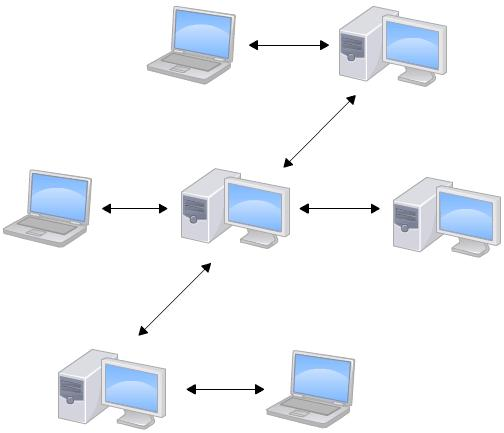
\includegraphics[scale = 0.7]{FenBuShi.jpg}
		  	\caption{分布式架构结构图}
		  \end{figure}
		  
		 当然,Git的优势不单是不必联网这么简单,后面我们还会看到Git极其强大的分支管理,把SVN等远远抛在了后面。
  \chapter{Git 安装配置}
  
  \chapter{Git 工作流程}
	  一般工作流程如下:
		  \begin{figure}[h]
		  	\centering
		  	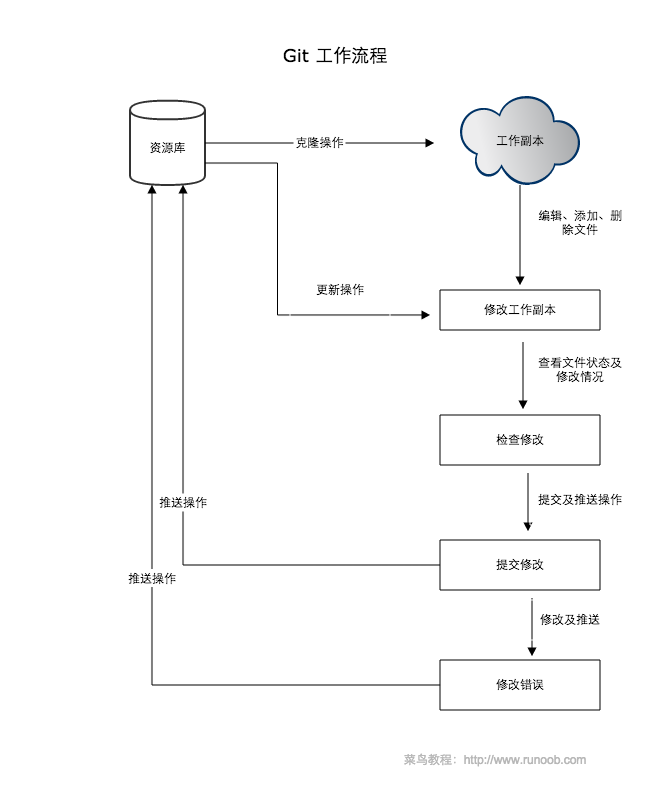
\includegraphics[scale = 0.5]{git-process.png}
		  	\caption{Git 工作流程图}
		  \end{figure}
		  
	  \begin{enumerate}
	  	\item \textbf{克隆} Git 资源作为工作目录
	  	\item \textbf{在克隆的资源上添加或修改文件}
	  	\item 如果其他人修改了,你可以更新资源
	  	\item \textbf{在提交前查看修改}
	  	\item 提交修改
	  	\item 在修改完成后,如果发现错误,可以撤回提交并再次修改并提交
	  \end{enumerate}
	  
  \chapter{Git 工作区、暂存区、版本库}
	  \section{版本库 repository}
		  什么是版本库呢?版本库又名仓库,英文名repository,\textbf{你可以简单理解成一个目录},\textit{这个目录里面的所有文件都可以被Git管理起来},\textbf{每个文件的修改、删除,Git都能跟踪},以便任何时刻都可以追踪历史,\textbf{或者在将来某个时刻可以“还原”}。
		  
		  工作区有一个隐藏目录.git,这个是Git的版本库
	  \section{工作区}
		  就是你在电脑里能看到的目录
		  
	  \section{暂存区}
		  英文叫stage, 或index。一般存放在 ".git目录下" 下的index文件(.git/index)中,所以我们把暂存区有时也叫作索引(index)
		  
	  \section{结构图}
	  
		  \begin{figure}[h]
		  	\centering
		  	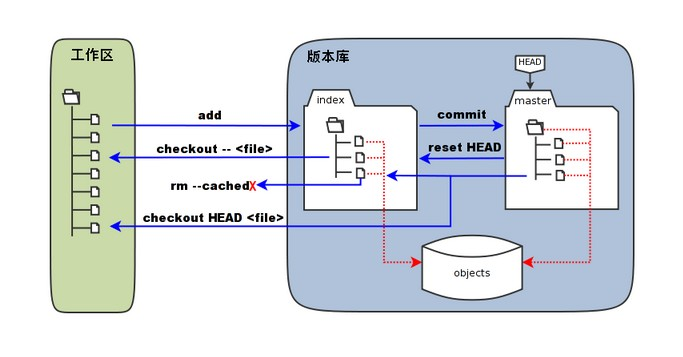
\includegraphics[scale = 0.8]{git-arc.jpg}
		  	\caption{Git 工作结构图}
		  \end{figure}
		  
		  \begin{itemize}
		  	\item 图中左侧为\textbf{工作区},右侧为\textbf{版本库}。在\textbf{版本库中}标记为 "index" 的区域是\textbf{暂存区}(stage, index),标记为 "master" 的是 master 分支所代表的目录树
		  	
		  	\item 图中我们可以看出此时 "HEAD" 实际是指向 master 分支的一个"游标"。所以图示的命令中出现 HEAD 的地方可以用 master 来替换。
		  	
		  	\item 图中的 objects 标识的区域为 Git 的\textbf{对象库},实际位于 "\verb|.git/objects|" 目录下,里面包含了创建的各种对象及内容
		  	\item 当对工作区修改(或新增)的文件执行 "\verb|git add|" 命令时,\textbf{暂存区}的目录树被更新,同时工作区修改(或新增)的文件内容\textbf{被写入到对象库中}的一个新的对象中,而\textbf{该对象的ID被记录在暂存区}的文件索引中
		  	
		  	\item 当执行提交操作(\verb|git commit|)时,\textbf{暂存区的目录树写到版本库(对象库)中},master 分支会做相应的更新。即 master 指向的目录树就是提交时暂存区的目录树
		  	
		  	\item 当执行 "\verb|git reset HEAD|" 命令时,暂存区的目录树会被重写,\textbf{被 master 分支指向的目录树所替换},但是工作区不受影响
		  	
		  	\item 当执行 "\verb|git rm --cached <file>|" 命令时,会直接从暂存区删除文件,工作区则不做出改变
		  	\item 当执行 "\verb|git checkout| ." 或者 "\verb|git checkout -- <file>|" 命令时,会\textbf{用暂存区}全部或指定的文件\textbf{替换工作区的文件}。这个操作很危险,会清除工作区中未添加到暂存区的改动
		  	
		  	\item 当执行 "\verb|git checkout HEAD| ." 或者 "\verb|git checkout HEAD <file>|" 命令时,\textbf{会用 HEAD 指向的 master 分支中的全部或者部分文件替换暂存区和以及工作区中的文件}。这个命令也是极具危险性的,因为不但会清除工作区中未提交的改动,也会清除暂存区中未提交的改动。 
		  \end{itemize}
  \chapter{Git 创建仓库}
	\section{git init}
		  Git 使用 \verb|git init| 命令来\textbf{初始化一个 Git 仓库},Git 的很多命令都需要在 Git 的仓库中运行,所以 \verb|git init| 是使用 Git 的第一个命令。
		  
		  在执行完成 \verb|git init| 命令后,Git 仓库会生成一个 \verb|.git 目录|,该目录包含了资源的所有元数据,其他的项目目录保持不变(不像 SVN 会在每个子目录生成 .svn 目录,\textbf{Git 只在仓库的根目录生成 .git 目录})。
		  \begin{lstlisting}
	// 使用当前目录作为Git仓库,我们只需使它初始化。该命令执行完后会在当前目录生成一个 .git 目录。现在在你的项目中生成了 .git 这个子目录。 这就是你的 Git 仓库了,所有有关你的此项目的快照数据都存放在这里。
	git init
	// 使用我们指定目录作为Git仓库。 
	git init newrepo
	// 初始化后,会在 newrepo 目录下会出现一个名为 .git 的目录,所有 Git 需要的数据和资源都存放在这个目录中。
	如果当前目录下有几个文件想要纳入版本控制,需要先用 git add 命令告诉 Git 开始对这些文件进行跟踪,然后提交: 
	$ git add *.c
	$ git add README
	$ git commit -m '初始化项目版本'
	//以上命令将目录下以 .c 结尾及 README 文件提交到仓库中。
		  \end{lstlisting}
		
	\section{git clone}
		我们使用 \verb|git clone| 从现有 Git 仓库中拷贝项目:\verb|git clone <repo> <directory>|
			\begin{itemize}[itemindent = 1em]
				\item \textbf{repo}:Git 仓库
				\item \textbf{directory}:本地目录
			\end{itemize}
		 
		 \begin{lstlisting}
	//比如,要克隆 Ruby 语言的 Git 代码仓库 Grit,可以用下面的命令: 
	$ git clone git://github.com/schacon/grit.git
	
	//执行该命令后,会在当前目录下创建一个名为grit的目录,其中包含一个 .git 的目录,用于保存下载下来的所有版本记录。 
	如果要自己定义要新建的项目目录名称,可以在上面的命令末尾指定新的名字:
	
	$ git clone git://github.com/schacon/grit.git mygrit
		 \end{lstlisting} 
  \chapter{Git 基本操作}
	  \section{基本操作}
		  \subsection{git status}
			  命令可以让我们时刻\textbf{掌握仓库当前的状态},得知添加到缓存中的文件是否被修改过了,是否是还没有准备提交的修改。例子结合\verb|git add| 一起学习。
			  
			  加上 \verb|-s| 参数,以获得简短的结果输出。如果没加该参数会详细输出内容
			  \begin{lstlisting}
	$ git status
	On branch master
	
	Initial commit
	
	Changes to be committed:
	(use "git rm --cached <file>..." to unstage)
	
	new file:   README
	new file:   hello.php
			  \end{lstlisting}
			  
		  \subsection{git add}
			  使用 \verb|git add |命令将想要\textbf{快照的内容写入缓存区}.
		  
			  \verb|git add| 命令可将该文件添加到缓存,如我们添加以下两个文件,	新项目中,添加所有文件很普遍,我们可以使用 \verb|'git add .'| 命令来添加当前项目的所有文件
			  \begin{lstlisting}
	$ touch README
	$ touch hello.php
	$ ls
	README		hello.php
	
	$ git status -s
	?? README
	?? hello.php
	$ 
	
	$ git add README hello.php 
	
	$ git status -s
	A  README
	A  hello.php
	$ 
	
	//现在我们修改 README 文件:
	$ vim README
	//在 README 添加以下内容:# Runoob Git 测试,然后保存退出。
	
	$ git status -s
	AM README
	A  hello.php
	
	//"AM" 状态的意思是,这个文件在我们将它添加到缓存之后又有改动。改动后我们在执行 git add 命令将其添加到缓存中
	$ git add .
	$ git status -s
	A  README
	A  hello.php
			  \end{lstlisting}
		\subsection{git diff}
			执行 \verb|git diff| 来\textbf{查看}执行 \verb|git status| 的结果的\textbf{详细信息}。
			
			\verb|git diff| 命令\textit{显示}\textbf{已写入缓存}与\textbf{已修改但尚未写入缓存的改动}的区别。\verb|git diff| 有两个主要的应用场景。
			
			\begin{itemize}
				\item 尚未缓存的改动:\verb|git diff| 
				\item 查看已缓存的改动: \verb|git diff --cached| 
				\item 查看已缓存的与未缓存的所有改动:\verb|git diff HEAD| 
				\item 显示摘要而非整个 diff:\verb|git diff --stat| 
			\end{itemize}
			
			\begin{lstlisting}
	// Example:
	// 在 hello.php 文件中输入以下内容:
	<?php
	echo '菜鸟教程:www.runoob.com';
	?>
	$ git status -s
	A  README
	AM hello.php
	$ git diff
	diff --git a/hello.php b/hello.php
	index e69de29..69b5711 100644
	--- a/hello.php
	+++ b/hello.php
	@@ -0,0 +1,3 @@
	+<?php
	+echo '菜鸟教程:www.runoob.com';
	+?>
			\end{lstlisting}
			
		\verb|git status| 显示你上次提交更新后的更改或者写入缓存的\textbf{改动}, 而 \verb|git diff| 一行一行地显示\textbf{这些改动具体是啥}
			
		\verb|git diff --cached| 的执行效果如下..具体体现缓存中的文件的更新时间戳与改动内容:
			\begin{lstlisting}
	$ git add hello.php 
	$ git status -s
	A  README
	A  hello.php
	$ git diff --cached
	diff --git a/README b/README
	new file mode 100644
	index 0000000..8f87495
	--- /dev/null
	+++ b/README
	@@ -0,0 +1 @@
	+# Runoob Git 测试
	diff --git a/hello.php b/hello.php
	new file mode 100644
	index 0000000..69b5711
	--- /dev/null
	+++ b/hello.php
	@@ -0,0 +1,3 @@
	+<?php
	+echo '菜鸟教程:www.runoob.com';
	+?>
			\end{lstlisting}
		\subsection{git commit}
			使用 \verb|git add |命令将想要\textbf{快照的内容写入缓存区}, 而执行 \verb|git commit| \textbf{将缓存区内容添加到仓库中}。

			Git 为你的每一个提交都记录你的名字与电子邮箱地址,所以第一步需要配置用户名和邮箱地址。
			\begin{lstlisting}
	$ git config --global user.name 'runoob'
	$ git config --global user.email test@runoob.com
			\end{lstlisting}
						
			接下来我们写入缓存,并提交对 hello.php 的所有改动。在首个例子中,我们使用 \verb|-m| 选项以在命令行中提供提交注释。
			\begin{lstlisting}
	$ git add hello.php
	$ git status -s
	A  README
	A  hello.php
	$ $ git commit -m '第一次版本提交'
	[master (root-commit) d32cf1f] 第一次版本提交
	2 files changed, 4 insertions(+)
	create mode 100644 README
	create mode 100644 hello.php
	
	$ git status
	# On branch master
	nothing to commit (working directory clean)
			\end{lstlisting}
			
			如果你觉得 \verb|git add |提交缓存的流程太过繁琐,Git 也允许你用 \verb|-a |选项跳过这一步。命令格式如下:\verb|git commit -a|
			\begin{lstlisting}
	// 我们先修改 hello.php 文件为以下内容:
	<?php
	echo '菜鸟教程:www.runoob.com';
	echo '菜鸟教程:www.runoob.com';
	?>
	// 再执行以下命令:
	git commit -am '修改 hello.php 文件'
	[master 71ee2cb] 修改 hello.php 文件
	1 file changed, 1 insertion(+)
			\end{lstlisting}
			
		\subsection{git rm}
		
		\subsection{git mv}
		
		
	\section{版本回滚与前进控制}
		\subsection{git log}
			在使用 Git 提交了若干更新之后,又或者克隆了某个项目,想回顾下提交历史,我们可以使用 \verb|git log| 命令查看。
			
			我们可以用 \verb|--oneline| 选项来查看历史记录的简洁的版本-告诉我们\textbf{此项目的开发历史}。
			\begin{lstlisting}
	$ git log --oneline
	88afe0e Merge branch 'change_site'
	14b4dca 新增加一行
	d7e7346 changed the site
	556f0a0 removed test2.txt
	2e082b7 add test2.txt
	048598f add test.txt
	85fc7e7 test comment from w3cschool.cc
			\end{lstlisting}
			
			我们还可以用 \verb|--graph| 选项,查看历史中什么时候出现了分支、合并。以下为相同的命令,开启了拓扑图选项,们可以\textbf{更清楚明了地看到何时工作分叉、又何时归并}
			\begin{lstlisting}
	$ git log --oneline --graph
	*   88afe0e Merge branch 'change_site'
	|\  
	| * d7e7346 changed the site
	* | 14b4dca 新增加一行
	|/  
	* 556f0a0 removed test2.txt
	* 2e082b7 add test2.txt
	* 048598f add test.txt
	* 85fc7e7 test comment from w3cschool.cc
			\end{lstlisting}
			
			可以用 '\verb|--reverse|'参数来\textbf{逆向显示所有日志}。
			\begin{lstlisting}
	$ git log --reverse --oneline
	85fc7e7 test comment from w3cschool.cc
	048598f add test.txt
	2e082b7 add test2.txt
	556f0a0 removed test2.txt
	d7e7346 changed the site
	14b4dca 新增加一行
	88afe0e Merge branch 'change_site'
			\end{lstlisting}
			
			如果只想\textbf{查找指定用户的提交日志}可以使用命令:\verb|git log --author| , 例如,比方说我们要找 Git 源码中 Linus 提交的部分
			\begin{lstlisting}
	$ git log --author=Linus --oneline -5
	81b50f3 Move 'builtin-*' into a 'builtin/' subdirectory
	3bb7256 make "index-pack" a built-in
	377d027 make "git pack-redundant" a built-in
	b532581 make "git unpack-file" a built-in
	112dd51 make "mktag" a built-in
			\end{lstlisting}
			
			如果\textbf{你要指定日期},可以执行几个选项:\verb|--since 和 --before|,但是你也可以用 \verb|--until 和 --after|。 
			例如,如果我要看 Git 项目中三周前且在四月十八日之后的所有提交,我可以执行这个(我还用了 \verb|--no-merges| 选项以隐藏合并提交)
			\begin{lstlisting}
	$ git log --oneline --before={3.weeks.ago} --after={2010-04-18} --no-merges
	5469e2d Git 1.7.1-rc2
	d43427d Documentation/remote-helpers: Fix typos and improve language
	272a36b Fixup: Second argument may be any arbitrary string
	b6c8d2d Documentation/remote-helpers: Add invocation section
	5ce4f4e Documentation/urls: Rewrite to accomodate transport::address
	00b84e9 Documentation/remote-helpers: Rewrite description
	03aa87e Documentation: Describe other situations where -z affects git diff
	77bc694 rebase-interactive: silence warning when no commits rewritten
	636db2c t3301: add tests to use --format="%N"
			\end{lstlisting}
		\subsection{git reset}
			需要友情提示的是,你看到的一大串类似\verb|3628164...882e1e0|的是\verb|commit id|(版本号)
			
			每提交一个新版本,实际上Git就会把它们自动串成一条时间线。如果使用可视化工具查看Git历史,就可以更清楚地看到提交历史的时间线
			
			首先,Git必须知道当前版本是哪个版本,在Git中,用\verb|HEAD|表示当前版本,也就是最新的提交\verb|3628164...882e1e0|(注意我的提交ID和你的肯定不一样),上一个版本就是\verb|HEAD^|,上上一个版本就是\verb|HEAD^^|,当然往上100个版本写100个\verb|^|比较容易数不过来,所以写成\verb|HEAD~100|。
			
			\subparagraph{-->即可以使用该命令回退到过去}现在,我们要把当前版本“\verb|append GPL|”回退到上一个版本“\verb|add distributed|”,就可以使用\verb|git reset|命令:
			\begin{lstlisting}
	$ git reset --hard HEAD^
	HEAD is now at ea34578 add distributed
			\end{lstlisting}
			
			此时,最新的那个版本\verb|append GPL|已经看不到了!-->\textbf{[可以通过 命令}\verb|git reflog| 来验证],好比你从21世纪坐时光穿梭机来到了19世纪,想再回去已经回不去了,肿么办?
			
			\subparagraph{-->用版本提交号码回到未来}办法其实还是有的,只要上面的命令行窗口还没有被关掉,你就可以顺着往上找啊找啊,找到那个\verb|append GPL|的\verb|commit id|是\verb|3628164...|,于是就可以指定回到未来的某个版本:
			
			\begin{lstlisting}
	$ git reset --hard 3628164
	HEAD is now at 3628164 append GPL
			\end{lstlisting}
  \chapter{Git 分支管理}
	  分支在实际中有什么用呢?假设你准备开发一个新功能,但是需要两周才能完成,第一周你写了50\%的代码,如果立刻提交,由于代码还没写完,不完整的代码库会导致别人不能干活了。如果等代码全部写完再一次提交,又存在丢失每天进度的巨大风险。
	  
	  现在有了分支,就不用怕了。你创建了一个属于你自己的分支,别人看不到,还继续在原来的分支上正常工作,而你在自己的分支上干活,想提交就提交,直到开发完毕后,再一次性合并到原来的分支上,这样,既安全,又不影响别人工作。
	  
	  使用分支意味着你可以从开发主线上分离开来,然后在不影响主线的同时继续工作。 
	  \section{分支基本操作}
		  \subsection{git branch (branchName)}
			  \textbf{创建分支},当直接使用\verb|git branch|时,它的意思是显示当前项目的所有分支,\textbf{但是加了后面的名字的话},如果没有的话就会创建一个新的分支出来
			  \begin{lstlisting}
	$ git branch
	* master
	
	$ git branch testing
	$ git branch
	* master
	  testing
			  \end{lstlisting}
		  \subsection{git checkout (branchName)}
			  \textbf{切换分支},当你切换分支的时候,Git 会用该分支的最后提交的快照替换你的工作目录的内容, 所以多个分支不需要多个目录
		  
			  用 \verb|git checkout (branch)| 切换到我们要修改的分支
			  \begin{lstlisting}
	$ ls
	README
	$ echo 'runoob.com' > test.txt
	$ git add .
	$ git commit -m 'add test.txt'
	[master 048598f] add test.txt
	2 files changed, 1 insertion(+), 3 deletions(-)
	delete mode 100644 hello.php
	create mode 100644 test.txt
	$ ls
	README		test.txt
	$ git checkout testing
	Switched to branch 'testing'
	$ ls
	README		hello.php
			  \end{lstlisting}
			  
			  当我们切换到"testing"分支的时候,我们添加的新文件test.txt被移除了, 原来被删除的文件hello.php文件又出现了。切换回"master"分支的时候,它们\textbf{又重新出现了}
			  \begin{lstlisting}
	$ git checkout master
	Switched to branch 'master'
	$ ls
	README		test.txt
			  \end{lstlisting}
		  \subsection{git branch -d (branchName)}
			 \textbf{删除分支},例如我们要删除"testing"分支
			  
			  \begin{lstlisting}
	$ git branch
	* master
	testing
	$ git branch -d testing
	Deleted branch testing (was 85fc7e7).
	$ git branch
	* master
			  \end{lstlisting}
		  \subsection{git merge}
			  你可以多次合并到统一分支, 也可以选择在合并之后直接删除被并入的分支,一旦某分支有了独立内容,你终究会希望将它合并回到你的主分支。 你可以使用以下命令将任何分支合并到当前分支中去
			  
			  \begin{lstlisting}
	$ git branch
	* master
	newtest
	$ ls
	README		test.txt	test2.txt
	$ git merge newtest
	Updating 2e082b7..556f0a0
	Fast-forward
	test2.txt | 1 -
	1 file changed, 1 deletion(-)
	delete mode 100644 test2.txt
	$ ls
	README		test.txt
			  \end{lstlisting}
	  \section{解决冲突}
		  使用\verb|git diff| 发现冲突文件,手动改写后,然后使用普通文件的添加和提交\verb|git add,commit|
  
  \chapter{GitHub 远程仓库}
	  \section{远程硬盘仓库-GitHub}
		  \subparagraph{第1步:创建SSHKey}。在用户主目录下,看看有没有\verb|.ssh|目录,如果有,再看看这个目录下有没有\verb|id_rsa和id_rsa.pub|这两个文件,如果已经有了,可直接跳到下一步。如果没有,打开Shell(Windows下打开Git Bash),创建SSH Key
		  
		  \begin{lstlisting}
	$ ssh-keygen -t rsa -C "ctzhenghua@163.com"
		  \end{lstlisting}
		  
		  你需要把邮件地址换成你自己的邮件地址,然后一路回车,使用默认值即可,由于这个Key也不是用于军事目的,所以也无需设置密码
		  
		  如果一切顺利的话,可以在用户主目录里找到.ssh目录,里面有\verb|id_rsa和id_rsa.pub|两个文件,这两个就是SSH Key的秘钥对,\verb|id_rsa|是私钥,不能泄露出去,\verb|id_rsa.pub|是公钥,可以放心地告诉任何人。
		  
		  \subparagraph{第2步:添加key}登陆GitHub,打开“\verb|Account settings|”,“\verb|SSH Keys|”页面:
		  然后,点“\verb|Add SSH Key|”,填上任意Title,在\verb|Key|文本框里粘贴\verb|id_rsa.pub|文件的内容
		  
		  点“\verb|Add Key|”,你就应该看到已经添加的Key
		  
		  \subparagraph{Notice}
			  为什么GitHub需要SSH Key呢?因为GitHub需要识别出你推送的提交确实是你推送的,而不是别人冒充的,而Git支持SSH协议,所以,GitHub只要知道了你的公钥,就可以确认只有你自己才能推送。
			  
			  当然,GitHub允许你添加多个Key。假定你有若干电脑,你一会儿在公司提交,一会儿在家里提交,只要把每台电脑的Key都添加到GitHub,就可以在每台电脑上往GitHub推送了。
			  
			  最后友情提示,在GitHub上免费托管的Git仓库,任何人都可以看到喔(但只有你自己才能改)。所以,不要把敏感信息放进去。
			  
			  如果你不想让别人看到Git库,有两个办法,一个是交点保护费,让GitHub把公开的仓库变成私有的,这样别人就看不见了(不可读更不可写)。另\textbf{一个办法是自己动手,搭一个Git服务器,因为是你自己的Git服务器,所以别人也是看不见的}。这个方法我们后面会讲到的,相当简单,公司内部开发必备。
	  \section{添加远程库}
		  在github 网站上创建项目..
	  \section{从远程库克隆}
		  git clone git@github.com:ctzhenghua/C-NetworkPractice-Code.git
		  
		  
		  \subsection{创建项目的目录结构}
			  1 创建目录 
			  
			  2 \verb|find . -type d -empty -exec touch {}\ .gitignore;\|
			  
			  3 git add
			  
			  4 git commit
	  
	  \section{多人协作}
	  
  \chapter{Git 服务器搭建}
  
  \chapter{参考}
		  动手教程 \url{https://try.github.io/levels/1/challenges/13}
		  
		  菜鸟教程  \url{http://www.runoob.com/git/git-tutorial.html}
		  
		  廖雪峰教程 \url{http://www.liaoxuefeng.com/wiki/0013739516305929606dd18361248578c67b8067c8c017b000}
\end{document} 
 		    